\documentclass[25pt, a0paper, portrait]{tikzposter} %Options for format can be included here
\usepackage[]{amsmath}
\usepackage{helvet}
\renewcommand{\familydefault}{\sfdefault}

\definecolorstyle{Eucall}{%
  \definecolor{ECGreen}{HTML}{98CE7C}%
  \definecolor{ECYellow}{HTML}{F2E560}%
  \definecolor{ECYellowGreen}{HTML}{D6DA36}%
}%
{
  % Background Colors
  \colorlet{backgroundcolor}{white}
  \colorlet{framecolor}{black}
  % Title Colors
  \colorlet{titlefgcolor}{white}
  %\colorlet{titlebgcolor}{ECGreen!50!ECYellowGreen}
  \colorlet{titlebgcolor}{ECGreen}
  % Block Colors
  %\colorlet{blocktitlebgcolor}{ECGreen!50!ECYellowGreen}
  \colorlet{blocktitlebgcolor}{ECGreen}
  \colorlet{blocktitlefgcolor}{white}
  \colorlet{blockbodybgcolor}{white}
  \colorlet{blockbodyfgcolor}{black}
  % Innerblock Colors
  %\colorlet{innerblocktitlebgcolor}{ECYellowGreen!50!ECYellow}
  \colorlet{innerblocktitlebgcolor}{ECYellowGreen}
  \colorlet{innerblocktitlefgcolor}{black}
  \colorlet{innerblockbodybgcolor}{white}
  \colorlet{innerblockbodyfgcolor}{black}
  % Note colors
  \colorlet{notefgcolor}{black}
  %\colorlet{notebgcolor}{ECGreen!50!ECYellowGreen}
  \colorlet{notebgcolor}{ECGreen}
  \colorlet{noteframecolor}{black}
}

\definetitlestyle{Eucall}{%
    width=0.95\paperwidth, roundedcorners=30, linewidth=0.0cm, innersep=1cm,
    titletotopverticalspace=15mm, titletoblockverticalspace=20mm,
    titlegraphictotitledistance=0pt, titletextscale=1
}{%
    \begin{scope}[line width=\titlelinewidth, rounded corners=\titleroundedcorners]%
      \coordinate (bottomleft) at (\titleposleft+0.2\textwidth, \titleposbottom);%
      \coordinate (topright) at (\titleposright, \titlepostop);%
      \pgftext[right, x=\titleposleft+0.18\textwidth, y=0.5\titlepostop+0.5\titleposbottom]{
\includegraphics[width=0.18\textwidth]{eucall_logo}}%
      \draw[draw=none, left color=ECGreen, right color=ECYellowGreen](bottomleft) rectangle (topright);%
    \end{scope}%
}

\defineblockstyle{EucallLeft}{
    titlewidthscale=1, bodywidthscale=1, titleleft,
    titleoffsetx=0pt, titleoffsety=0pt, bodyoffsetx=25pt, %bodyoffsety=-10pt,
    bodyverticalshift=0pt, roundedcorners=30, linewidth=0.0cm,
    titleinnersep=1cm, bodyinnersep=1cm
}{%
    \begin{scope}[line width=\blocklinewidth, rounded corners=\blockroundedcorners]%
        \ifBlockHasTitle %
           \draw[draw=none, left color=ECGreen, right color=ECYellowGreen] (blocktitle.south west) rectangle (blocktitle.north east);
           \draw[draw=none, fill=blockbodybgcolor] (blockbody.south west) rectangle (blockbody.north east);
        \else
           \draw[draw=none, fill=blockbodybgcolor] (blockbody.south west) rectangle (blockbody.north east);
        \fi
    \end{scope}
}
\defineblockstyle{EucallCenter}{
    titlewidthscale=1, bodywidthscale=1, titleleft,
    titleoffsetx=0pt, titleoffsety=0pt, bodyoffsetx=25pt, bodyoffsety=-10pt,
    bodyverticalshift=0pt, roundedcorners=30, linewidth=0.0cm,
    titleinnersep=1cm, bodyinnersep=1cm
}{%
    \begin{scope}[line width=\blocklinewidth, rounded corners=\blockroundedcorners]%
        \ifBlockHasTitle %
           \draw[draw=none, fill=ECGreen] (blocktitle.south west) rectangle (blocktitle.north east);
           \draw[draw=none, fill=ECGreen] (blockbody.south west) rectangle (blocktitle.north east);
        \else
           \draw[draw=none, fill=blockbodybgcolor] (blockbody.south west) rectangle (blockbody.north east);
        \fi
    \end{scope}
}
\defineblockstyle{EucallRight}{
    titlewidthscale=1, bodywidthscale=1, titleleft,
    titleoffsetx=0pt, titleoffsety=0pt, bodyoffsetx=25pt, bodyoffsety=0pt,
    bodyverticalshift=0pt, roundedcorners=30, linewidth=0.0cm,
    titleinnersep=1cm, bodyinnersep=1cm
}{
    \begin{scope}[line width=\blocklinewidth, rounded corners=\blockroundedcorners]
        \ifBlockHasTitle %
           \draw[draw=none, left color=ECYellowGreen, right color=ECYellow] (blocktitle.south west) rectangle (blocktitle.north east);
           \draw[draw=none, color=blockbodybgcolor] (blockbody.south west) rectangle (blockbody.north east);
        \else
           \draw[draw=none, color=blockbodybgcolor] (blockbody.south west) rectangle (blockbody.north east);
        \fi
    \end{scope}
}



\definelayouttheme{Eucall}{%
  \usecolorstyle{Eucall}
  %\usecolorstyle{default}
  \usebackgroundstyle{Default}
  \usetitlestyle{Eucall}
  \useblockstyle{EucallLeft}
  \usenotestyle{Default}
}


% Switch off the tikz notice at the bottom
\tikzposterlatexaffectionproofoff

%%%%%%%%%%%%%%%%%%%%%%%%%%%%%%%%%%%%%%%%%%%%%%%%%%%%%%%%%%%%%%%%%%%%%%
%%% Begin of Document
%%%%%%%%%%%%%%%%%%%%%%%%%%%%%%%%%%%%%%%%%%%%%%%%%%%%%%%%%%%%%%%%%%%%%%


 % Title, Author, Institute
 \title{\hspace*{0.2\textwidth}\parbox{0.7\textwidth}{\centering\bf Simulation
 of Experiments in the European Cluster of Advanced Laser Light Sources}}
 \author{\hspace*{0.2\textwidth}{\parbox{0.7\textwidth}{\centering\normalsize%
 C. Fortmann-Grote$^\text{1}$,
 A. Andreev$^\text{2}$,
 A. Ashutosh$^\text{2}$
 R. Briggs$^\text{3}$,
 M. Bussmann$^\text{4}$,
 A. Buzmakov$^\text{5}$
 M. Garten$^\text{4}$,
 A. Grund$^\text{4}$,
 A. H\"ubl$^\text{4}$,
 Z. Jurek$^\text{6}$,
 N. D. Loh$^\text{7}$,
 S. Pascarelli$^\text{3}$,
 L. Samoylova$^\text{1}$,
 R. Santra$^\text{6}$,
 E. A. Schneidmiller$^\text{8}$,
 T. Tschentscher$^\text{1}$,
 S. Yakubov$^\text{8}$,
 C. H. Yoon$^\text{9}$,
 M. Yurkov$^\text{8}$,
 B. Ziaja$^\text{6}$,
 and A. P. Mancuso$^\text{1}$
 }}}
 \institute{\hspace*{0.2\textwidth}{\parbox{0.7\textwidth}{\centering\small%
 $^\text{1}$European XFEL, Hamburg, Germany,
 $^\text{2}$ELI-ALPS, Szeged, Hungary,
 $^\text{3}$ESRF, Grenoble, France,
 $^\text{4}$HZDR, Dresden, Germany,
 $^\text{5}$FSRC ``Crystallography and Photonics''  Russian Academy of Sciences, Moscow, Russia
 $^\text{6}$CFEL, Hamburg, Germany
 $^\text{7}$National University of Singapore, Singapore
 $^\text{8}$DESY, Hamburg, Germany,
 $^\text{9}$LCLS, Menlo Park, USA,
 }}}

 %Choose Layout
\usetheme{Eucall}

%Reference counter
\newcounter{refcounter}
\setcounter{refcounter}{1}

\newcommand{\getCounter}[1]{\arabic{#1}\stepcounter{#1}}
\begin{document}
%\begin{minipage}{.9\colwidth}%
  %\mbox{}%
  %\begin{minipage}[][.1\textheight][t]{.475\textwidth}%
    %\innerblock[titlewidth=\textwidth,bodywidth=\textwidth,titleleft, titleoffsetx=10pt,
    %bodyoffsetx=10pt]

% Title block with title, author, logo, etc.
\maketitle
%%%%%%%%%%%%%%% TOP ROW %%%%%%%%%%%%%%%%
\useblockstyle{Eucall}
\block[]{SIMEX: A generic simulation platform for photon science experiments
  [\getCounter{refcounter},\getCounter{refcounter}]}{%
  \begin{minipage}{.9\textwidth}%
    \mbox{}%
    \begin{minipage}[][][t]{.38\textwidth}
      \innerblock[titleleft]{Start--to--end simulations}{%
        \begin{center}%
          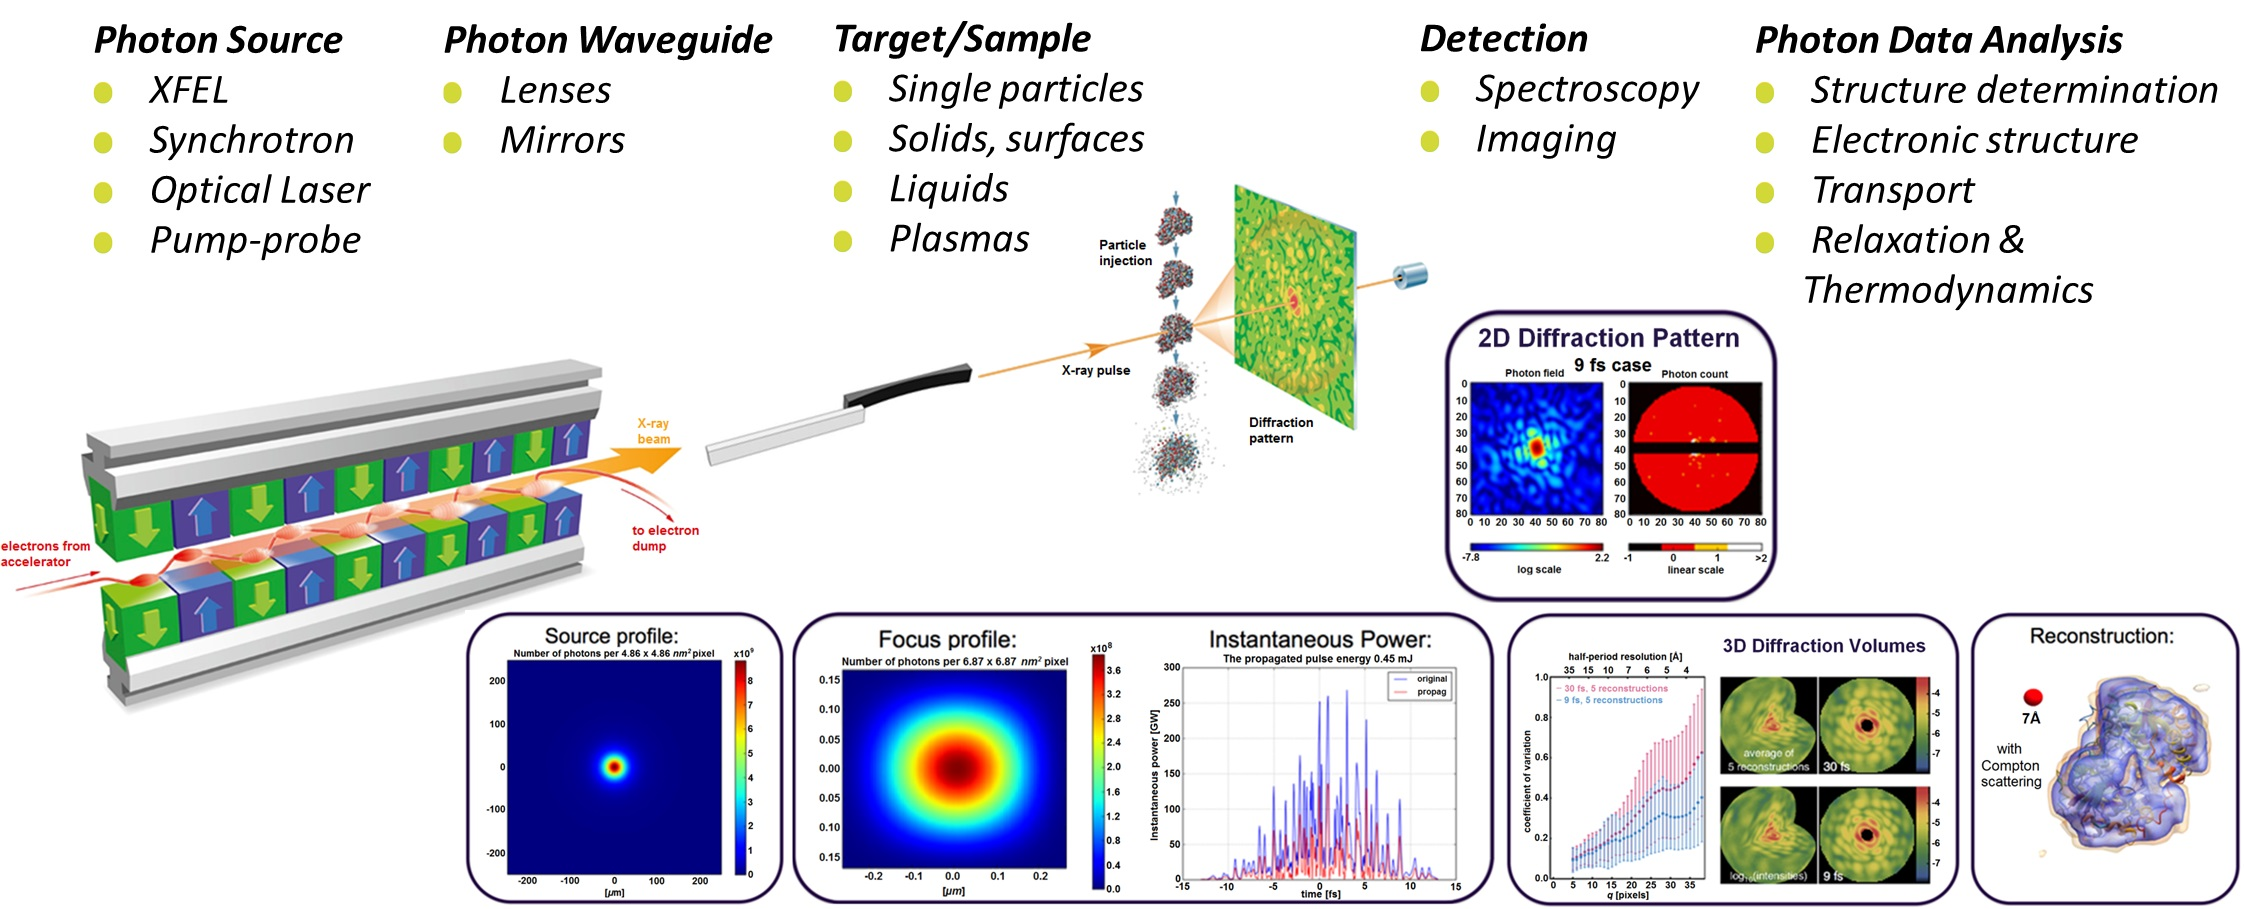
\includegraphics[width=0.9\textwidth,angle=0,clip]{simS2E_workflow}%
        \end{center}%
      }
    \end{minipage}%
    \hfill%
    \begin{minipage}[][][t]{.285\textwidth}
      \innerblock[titleleft]{Data flow in SIMEX}{%
        \begin{center}%
          \includegraphics[width=0.9\textwidth,angle=0,clip]{simex_workflow_slide-crop}%
        \end{center}%
      }
    \end{minipage}%
    \hfill%
    \begin{minipage}[][][t]{.205\textwidth}
      \innerblock[titleleft]{Python scripting}{%
        \begin{center}%
          \includegraphics[width=0.9\textwidth,angle=0,clip]{simex_script}%
        \end{center}%
      }
    \end{minipage}%
    \hfill%
    \begin{minipage}[][][t]{.1\textwidth}
      \innerblock[titleleft]{Standardized data format}{%
        \begin{center}%
          \includegraphics[width=0.42\textwidth,angle=0,clip]{opmd_screenshot}\\
          {\small www.openpmd.org}
        \end{center}%
      }
    \end{minipage}%
  \end{minipage}
}
\begin{columns}
%%%%%%%%%%%%%%% FIRST column
\column{0.5}%
%%%
\block[bodyoffsetx=20pt]{Single particle imaging of biomolecules
  [1,\getCounter{refcounter}]}{%
    \innerblock[titleleft]{Studying diffraction data quality as a function of x--ray pulse
        duration}
    {%
    \begin{minipage}[ ]{.9\colwidth}
      \mbox{}%
      \begin{minipage}[][][t]{.39\textwidth}
        \includegraphics[width=\textwidth,angle=0,clip]{single_particle_imaging_scheme_shaded_bg+2nip.png}\\
      {\small Sample molecule 2NIP}
    \end{minipage}
      \hfill%
      \begin{minipage}[][][t]{.59\textwidth}
        \sloppy
        \begin{itemize}
          \item XFEL source simulation: FAST code, XPD database xpd.xfel.eu
          \item X--ray pulse propagation: WPG/SRW [\getCounter{refcounter}]
          \item Sampling source fluctuations, sample orientation, and ionization
            dynamics $\Rightarrow$ 200000 simulated patterns
          \item Compare pulses of 3, 9, and 30 fs duration.
        \end{itemize}
    \end{minipage}
    \end{minipage}
    }%
    \innerblock[titleleft, titleoffsetx=10pt, bodyoffsetx=10pt]
    {Photon--matter interaction: XMDYN$\,$\&$\,$XATOM [\getCounter{refcounter}]}
    {%
      \begin{minipage}[ ]{.9\colwidth}
          \begin{center}
            \includegraphics[width=.32\textwidth,angle=0,clip]{pmi_3fs}%
            \includegraphics[width=.32\textwidth,angle=0,clip]{pmi_9fs}%
            \includegraphics[width=.32\textwidth,angle=0,clip]{pmi_30fs}\\
          \end{center}
      \end{minipage}
    }%
    \innerblock[titleleft, titleoffsetx=10pt, bodyoffsetx=10pt]
    {Reconstructed 3D diffraction volumes and coefficient of variation}
    {%
      \vspace*{2ex}
      \begin{minipage}[ ]{.9\colwidth}
          \begin{center}
            \mbox{}%
            \begin{minipage}[][][t]{.53\textwidth}
              \includegraphics[width=.99\textwidth,angle=0,clip]{scattering_vs_pulseduration}\\
              {\small Photon counts and scattering efficiency vs.
            pulse duration }
            \end{minipage}
            \begin{minipage}[][][t]{.43\textwidth}
              %\includegraphics[width=.9\textwidth,angle=0,clip]{diffr_orient_flow}
            \end{minipage}
            {\small%
            \begin{equation*}
               \sigma_\text{v}(q) = \frac{1}{M_q}\sum_{\mathbf{q}: |\mathbf{q}|=q} \frac{ \sqrt{\frac{1}{N} \sum_{i=1}^N \left( I_i(\mathbf{q}) - \langle I(\mathbf{q})\rangle_N \right)^2 } } { \langle I(\mathbf{q})\rangle_N }
               \label{eqn:coeff_variation}
             \end{equation*}
           }
           \hspace*{.05\textwidth}
             \includegraphics[width=.4\textwidth,angle=0,clip]{varcoeff_3-9-30-crop}%
            \hfill
            \includegraphics[width=.4\textwidth,angle=0,clip]{varcoeff_3scaled-9-crop}%
           \hspace*{.05\textwidth}
          \end{center}
        \end{minipage}\\[1ex]
    \textbf{Ultra--short 3 fs pulses do not contain enough photons to produce
      reliable diffraction data despite negligible radiation damage}
    }%
}
\column{0.5}
\useblockstyle{Eucall}
%%%%%%%%%%%%% HPL %%%%%%%%%%%%%
\block[bodyoffsetx=-20pt]{X-ray diffraction in solid density plasmas
  [\getCounter{refcounter}]}{%
    \innerblock[titleleft, titleoffsetx=10pt,bodyoffsetx=10pt]
    {Identifying plasma instabilities by small angle x-ray scattering}
    {%
    \begin{minipage}[ ]{.9\colwidth}
      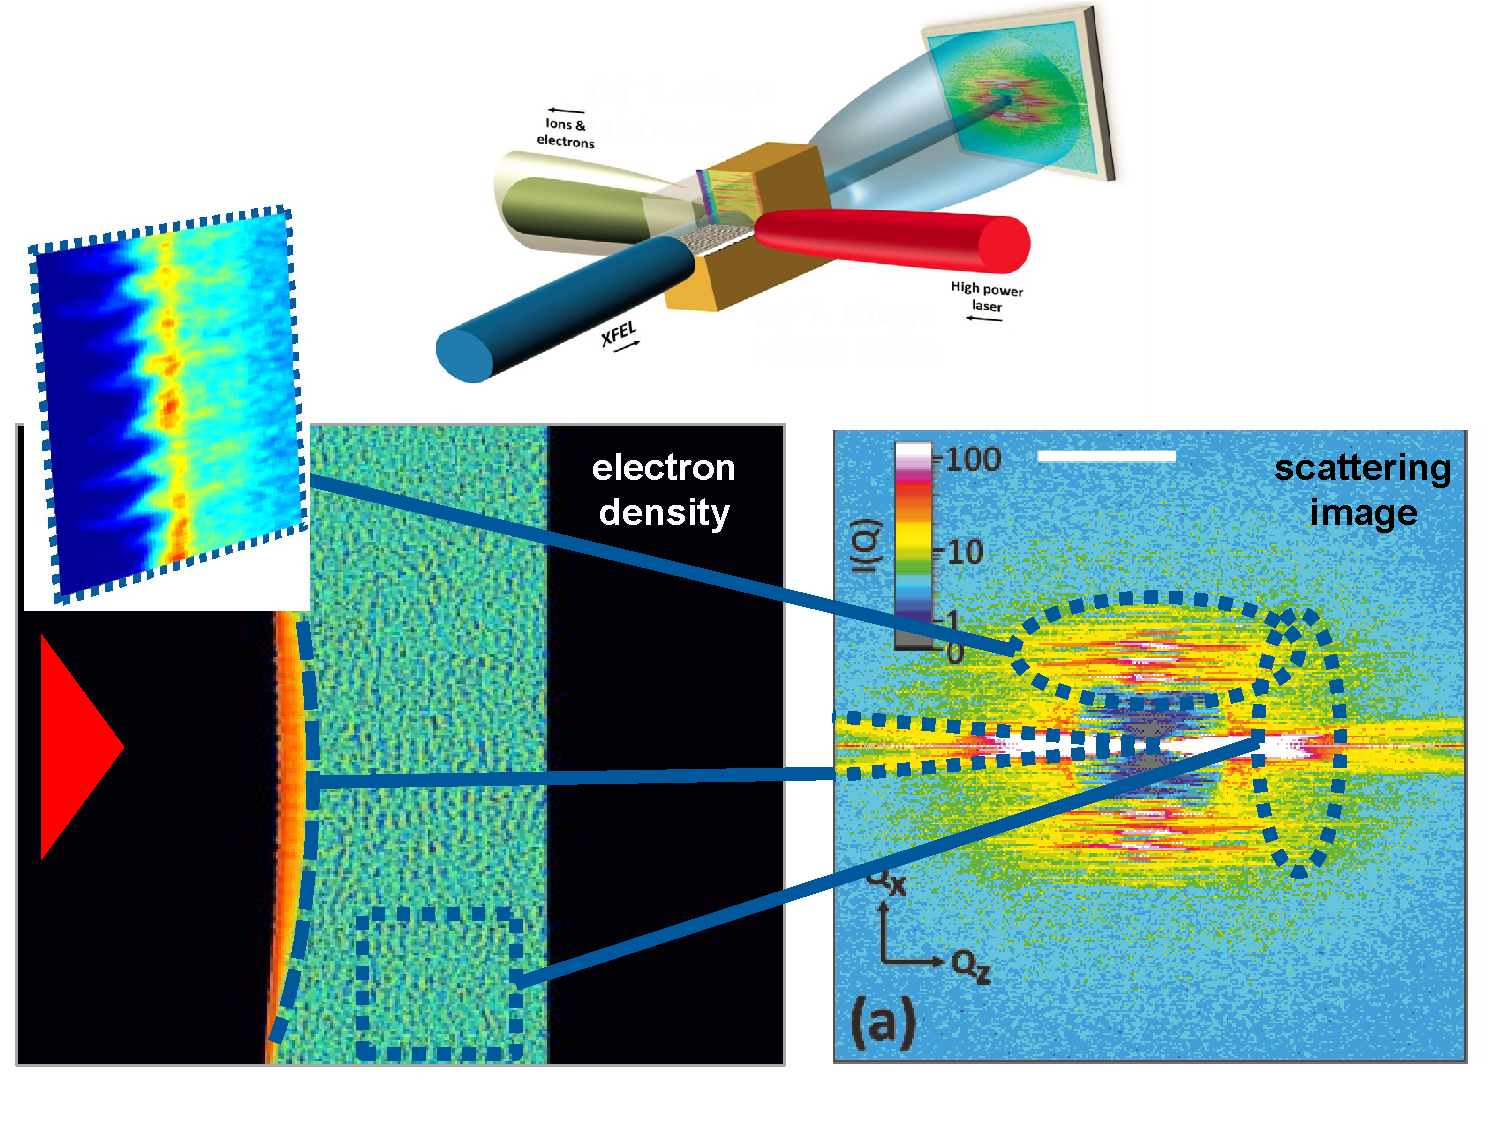
\includegraphics[width=.5\textwidth,angle=0,clip]{bussmann_saxs.pdf}%
      \hfill%
      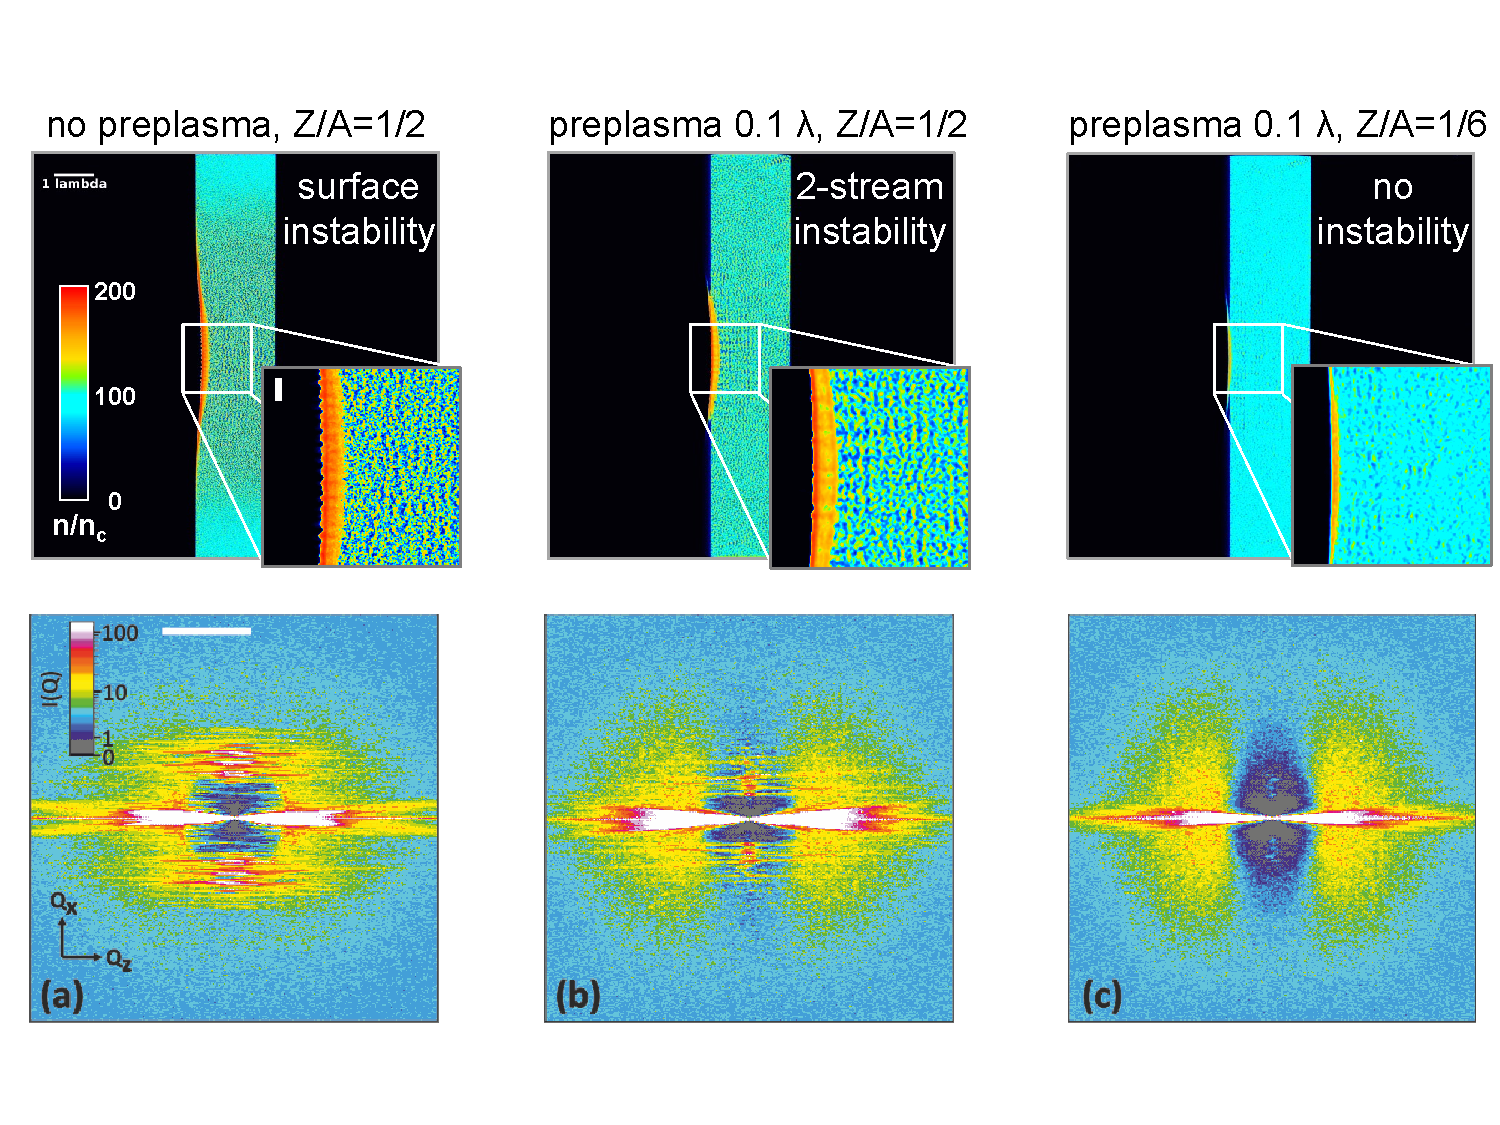
\includegraphics[width=.5\textwidth,angle=0,clip]{bussmann_saxs_instabilities.pdf}%
    \end{minipage}
    }%
    \innerblock[titleleft, titleoffsetx=10pt, bodyoffsetx=10pt]
    { Outlook: Combine PIC simulations [\getCounter{refcounter}] with population
    kinetics [\getCounter{refcounter}]}
    {%
      \begin{minipage}[ ]{.9\colwidth}
        \mbox{}%
        \begin{minipage}[][][t]{.49\textwidth}
          \begin{center}
            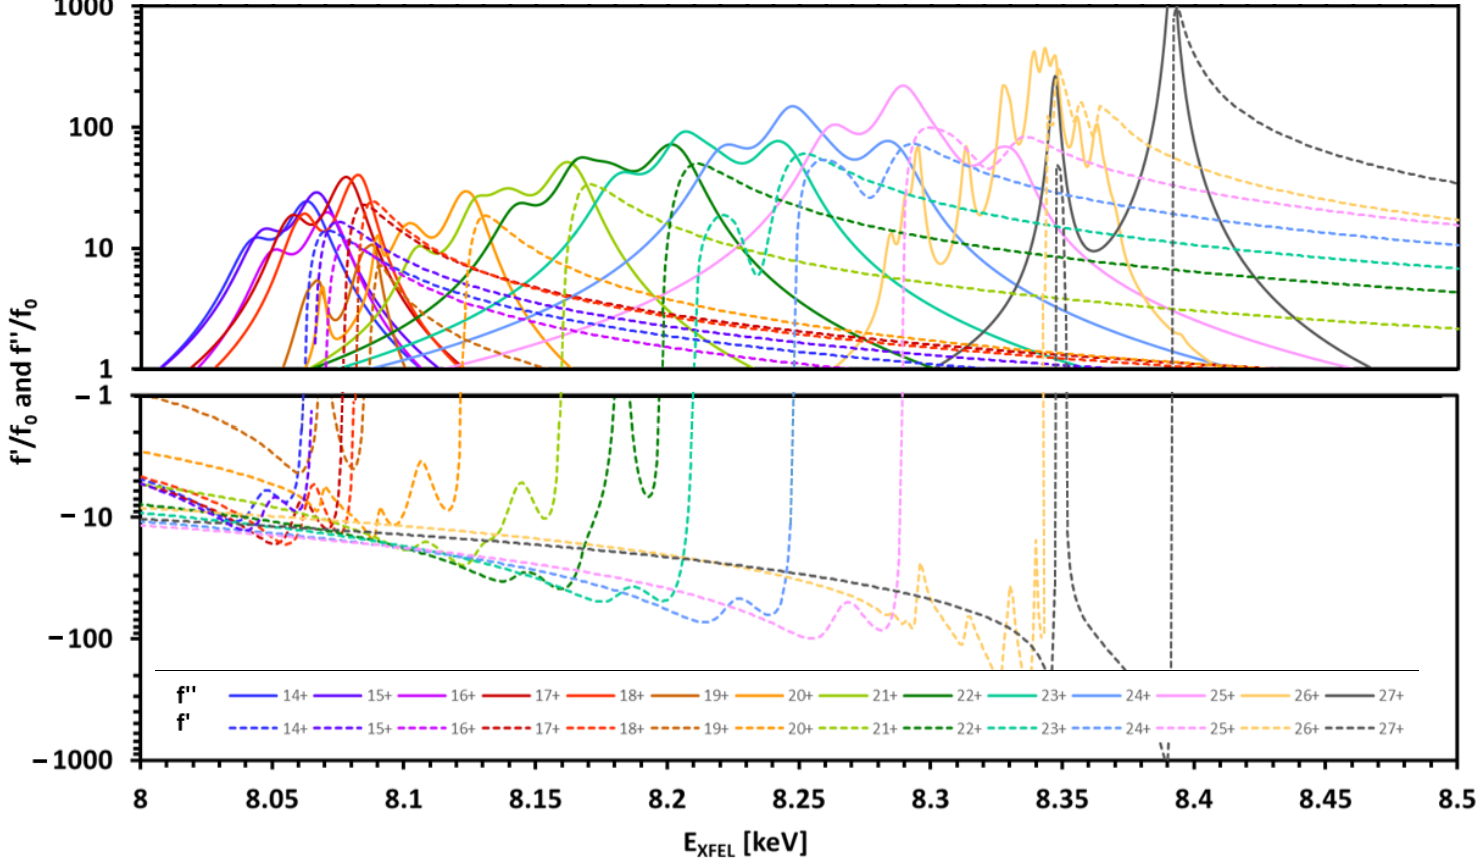
\includegraphics[width=.4\colwidth,angle=0,clip]{scfly.png}%
          \end{center}
        \end{minipage}
        \begin{minipage}[][][t]{.49\textwidth}
          \begin{itemize}
            \item Multiple photon scattering
            \item Atomic configurations
            \item Collisions
            \item Collisional and field ionization
            \item Radiation transport
            \item Recombination
          \end{itemize}
        \end{minipage}
      \end{minipage}
    }%
}%
%%%
% ESRF WDM Diagnostics
\block[bodyoffsetx=-10pt]{X-ray diagnostics of warm dense matter}{%
  \innerblock[titleleft, titleoffsetx=10pt, bodyoffsetx=10pt]{X-ray absorption
    spectroscopy in laser shock compressed iron [\getCounter{refcounter}]}{
  \begin{center}
    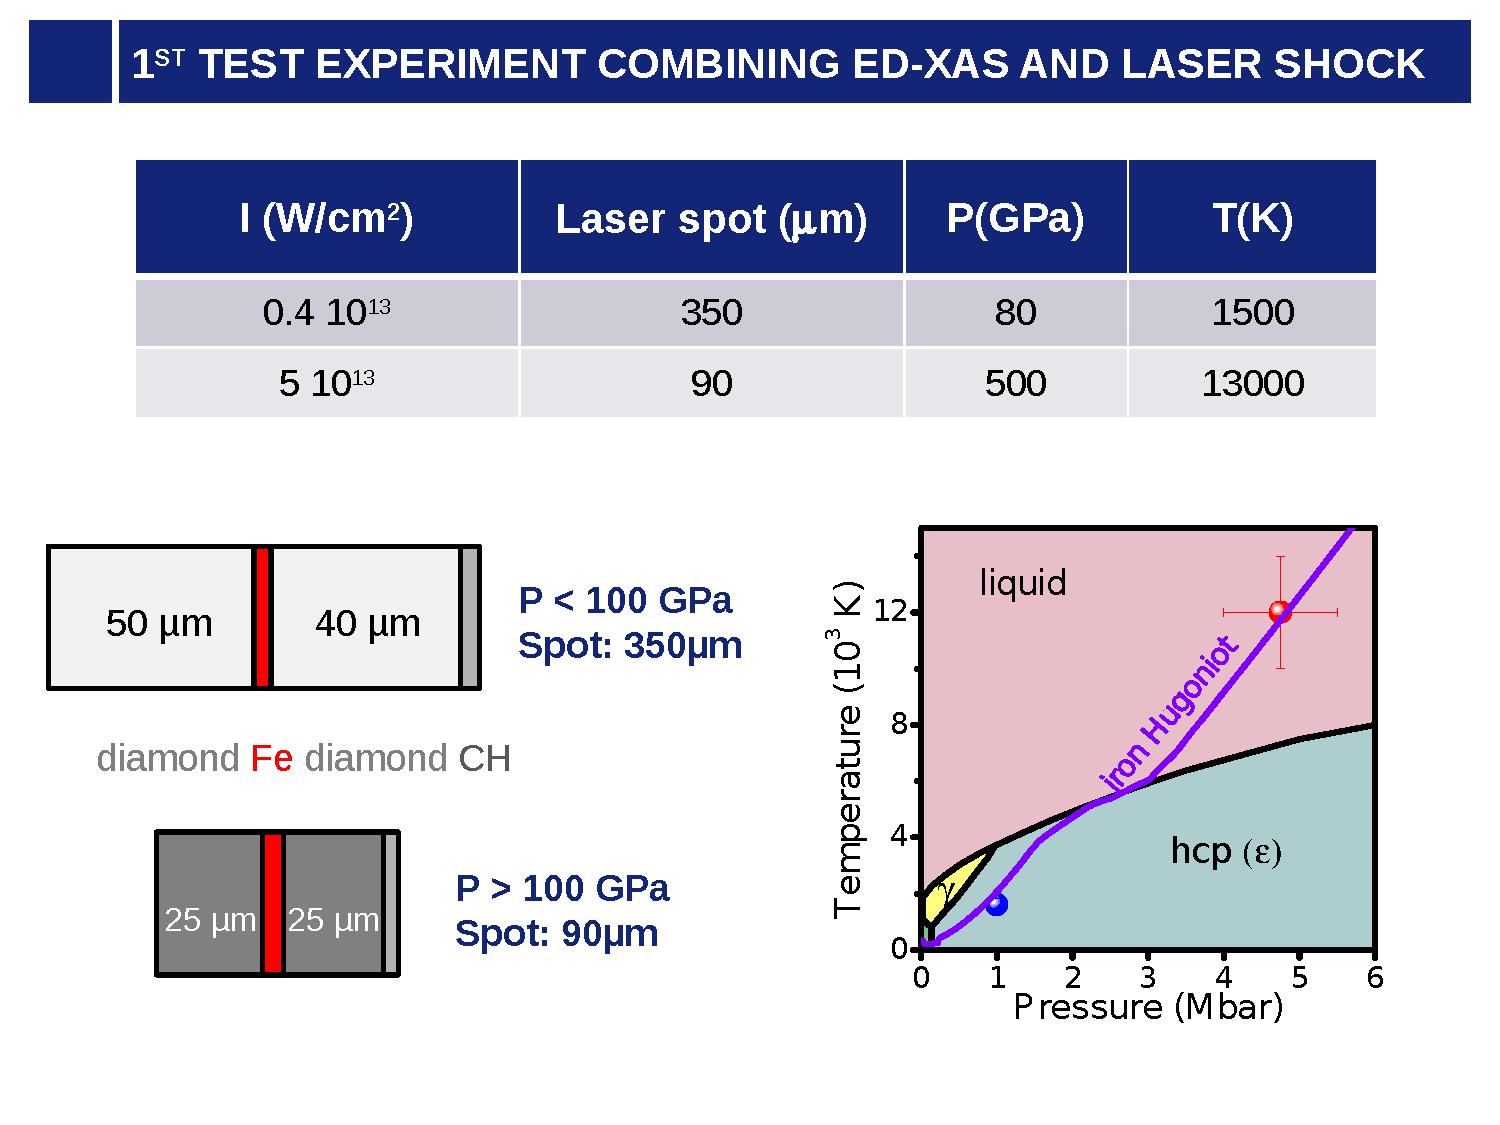
\includegraphics[width=0.45\colwidth,angle=0,clip, bb=0 0 700 470]{esrf_Fe_targets_eos}%
    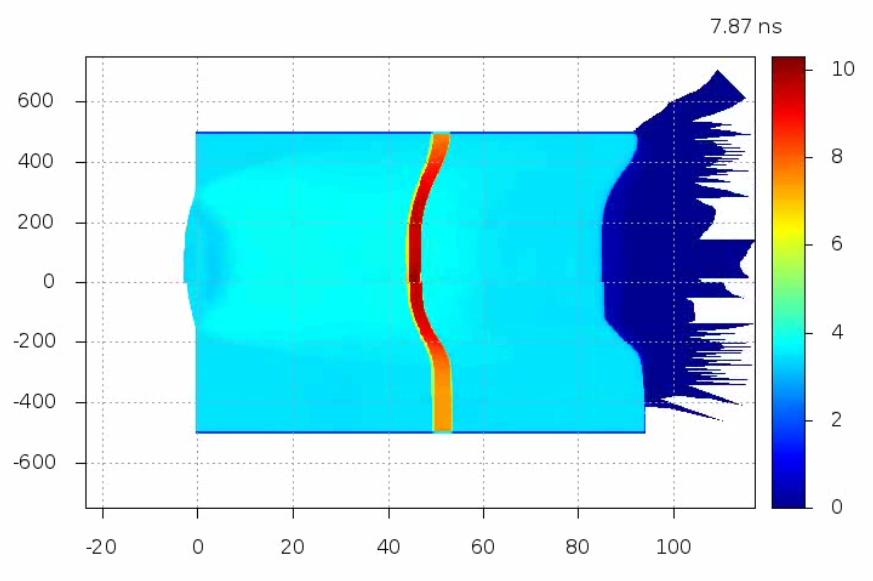
\includegraphics[width=0.45\colwidth,angle=0,clip]{esrf_Fe_sandwich_hydrosim}\\[2.8ex]
    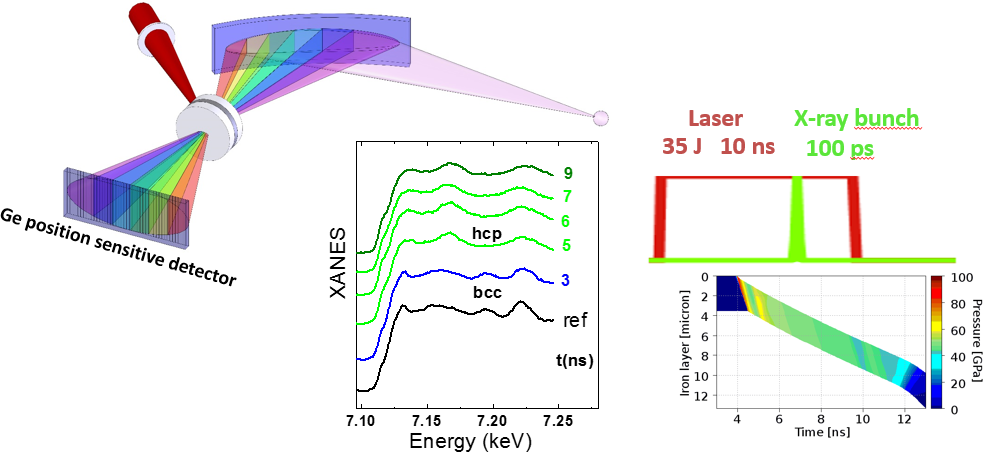
\includegraphics[width=0.88\colwidth,height=0.333\colwidth,angle=0,clip]{esrf_Fe_xas_position}
  \end{center}
  }
}
\end{columns}
%%%%%%%%%%%%% FOOTER %%%%%%%%%%%%%%%%%%%%%
\block{}{%
\vspace*{-4ex}
\begin{tikzpicture}%
  \draw (0,0) -- ( \textwidth - 4.5cm, 0);
\end{tikzpicture}\\[1ex]
\mbox{}
\begin{minipage}[][][t]{0.25\textwidth}%
  \noindent%
  {\sf%
  Contact: carsten.grote@xfel.eu\\%
  \noindent%
  Webpage: www.eucall.eu\\[2ex]
  }%
  \begin{minipage}{\textwidth}
    \mbox{}%
    \begin{minipage}[][][t]{0.2\textwidth}%
      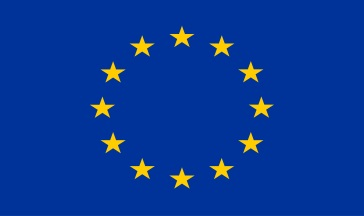
\includegraphics[width=1.0\textwidth]{eu-flag}%
    \end{minipage}%
    \hfill%
    \begin{minipage}[][][t]{0.79\textwidth}%
    \small%
    This project has received funding from the \textit{European Union's Horizon 2020 research and
    innovation programme} under grant agreement No 654220.
    \end{minipage}%
  \end{minipage}
\end{minipage}%
\hfill%
\begin{minipage}[][][t]{0.35\textwidth}%
  \includegraphics[width=\textwidth,angle=0,clip]{eucall_institutes}%
\end{minipage}%
\hspace*{10pt}%
\begin{minipage}[][][t]{0.34\textwidth}
  \small
  %\setlength{\baselineskip}{2pt}
  \begin{enumerate}
    \item Yoon et al. Sci. Reports \textbf{6} (2016).
    \item Fortmann-Grote et al. J. Phys. Conf. Series (accepted),
      arXiv:1610.05980.
    \item Fortmann-Grote et al. (submitted).
    \item Samoylova et al. J. Appl Cryst. \textbf{49} (2016).
    \item Jurek et al.  J. Appl Cryst. \textbf{49} (2016).
    \item Kluge et al. Phys. Plasma \textbf{23} (2016).
    \item Burau et al. IEEE Trans. Plasma Sc. \textbf{38} (2010); http://picongpu.hzdr.de.
    \item Chung et al, HEDP \textbf{1} (2005).
    \item Torchio et al., Sci. Reports \textbf{6} (2016).
  \end{enumerate}
\end{minipage}
}
\end{document}



